\documentclass{article}
\usepackage{spconf,amsmath,amssymb,graphicx,booktabs,multirow,xcolor}
\usepackage[hidelinks]{hyperref}
\usepackage{enumitem}
\setlist{nosep, leftmargin=12pt}
\newcommand{\ff}{\mathrm{FF}}

\title{Smaller looks rounder: resolution-dependent bias of shape descriptors in open-source bioimage and radiomics software}
\name{Anonymous Author(s)}
\address{Affiliation}

\begin{document}
\maketitle

\begin{abstract}
Circularity and sphericity are ubiquitous shape descriptors in cell morphometry and radiomics, yet their values depend on how the software estimates the perimeter or surface area of a mask. We audit eight implementations, including scikit-image (hence CellProfiler), OpenCV, ImageJ and PyRadiomics/IBSI, against exact ground truth and derive a closed-form model of their bias. The default 2D estimators make the same object rounder the fewer pixels it covers, and the IBSI sphericity of a sphere drops from $0.92$ to $0.82$ as CT slices thicken from 1 to 5\,mm; isotropic resampling makes it worse. On nuclei re-segmented with Cellpose at several resolutions, halving the magnification shifts the default form factor by $0.7$--$0.95$ standard deviations. In PanNuke, the default estimator nearly doubles the roundness difference between inflammatory and tumour nuclei, reverses the sign of another contrast at $10\times$, and inflates it 4.6-fold when scanners are mixed. A one-line correction of existing feature tables and a spacing-aware 3D Crofton estimator remove most of these errors.
\end{abstract}

\begin{keywords}
Morphometry, radiomics, harmonization, digital geometry, reproducibility
\end{keywords}

\section{Introduction}
\label{sec:intro}
Shape descriptors of segmented objects are a staple of quantitative imaging. Nuclear circularity quantifies pleomorphism in histopathology, CellProfiler's \emph{FormFactor} is part of every Cell Painting profile~\cite{bray2016,stirling2021}, and sphericity is a standardized radiomics feature of the Image Biomarker Standardisation Initiative (IBSI)~\cite{zwanenburg2020}. Both are ratios of a size to a boundary measure, $\ff=4\pi A/P^2$ and $\Psi=(36\pi V^2)^{1/3}/S$, equal to $1$ for a disk and a ball. Studies routinely pool data of different resolution: whole-slide images scanned at $20\times$ and $40\times$, cells of different sizes, CT series with 1--5\,mm slices.

The area or volume of a mask is easy to estimate, since the pixel count is unbiased under random placement. The boundary is not: digital geometry has long shown that local perimeter estimators are biased and do not converge as the resolution increases~\cite{kulpa1977,lindblad2005}. Kulpa~\cite{kulpa1977} derived the large-object length factor $\kappa$ of chain codes; Crofton estimators avoid it~\cite{legland2007}; and MATLAB patched its circularity for small objects in 2023~\cite{matlab2023}. What is missing is (a) a model of the \emph{size dependence} of the estimators actually shipped in open-source tools, which is what breaks comparisons across resolutions, (b) evidence of how large the effect is in real pipelines, and (c) fixes that also repair data already analysed.

\noindent\textbf{Contributions.} (i) A closed-form model $P\approx\kappa(L-2\pi\delta)$ with a new offset term $\delta=\sqrt2/\pi$ that predicts the size dependence of the default estimators (Fig.~\ref{fig:main}b). (ii) An audit of eight 2D/3D implementations against exact ground truth. (iii) Evidence on 66k annotated and 23k independently re-segmented nuclei and on lung tumours: resolution shifts, distorted biological contrasts, and degraded cross-resolution classification. (iv) Fixes: a post-hoc correction F1 that repairs existing feature tables without the masks; in 3D, we show that a spacing-aware Crofton estimator (F3) on the native grid removes the slice-thickness bias of IBSI sphericity, whereas IBSI's recommended isotropic resampling does not.

\section{Bias model and fixes}
\label{sec:model}
Let $X\subset\mathbb{R}^2$ have a smooth boundary of length $L$, digitized on a unit grid as $D=X\cap\mathbb{Z}^2$ (pixels whose centres lie in $X$) with random sub-pixel position and orientation. Most estimators trace a polygon along $D$ whose edges take a few lattice directions (Fig.~\ref{fig:main}a). Let a boundary element of length $ds$ and tangent angle $\theta$ be represented by polygon length $g(\theta)\,ds$, and let the polygon lie on average a distance $\delta$ inside $\partial X$. By Steiner's formula, a closed curve moved inward by $\delta$ has length $L-2\pi\delta$; averaging $g$ over orientations then gives
\begin{equation}
P \approx \kappa\,(L-2\pi\delta),\qquad \kappa=\tfrac{1}{2\pi}\textstyle\int_0^{2\pi} g(\theta)\,d\theta .
\label{eq:model}
\end{equation}
\emph{Chain codes}, used by scikit-image's default \texttt{regionprops} perimeter (hence CellProfiler), by OpenCV's \texttt{arcLength} and by MATLAB up to R2022b, join the centres of the boundary pixels (object pixels with a background 4-neighbour) by horizontal, vertical or diagonal steps of length $1$ or $\sqrt2$. Thus $g(\theta)=|\cos\theta|+(\sqrt2-1)|\sin\theta|$ for $|\theta|\le\pi/4$ and $\kappa=8(\sqrt2-1)/\pi\approx1.0548$~\cite{kulpa1977}. Along the grid axis closest to the boundary normal, the last pixel centre inside $X$ lies at a uniform distance in $[0,1)$ from $\partial X$, i.e.\ $\cos\theta/2$ on average perpendicular to it, so $\delta=\tfrac{4}{\pi}\int_0^{\pi/4}\tfrac{\cos\theta}{2}d\theta=\sqrt2/\pi\approx0.45$. For a disk of radius $r$ pixels,
\begin{equation}
\ff_{\text{chain}}(r)\approx \kappa^{-2}\,\big(r/(r-\sqrt2/\pi)\big)^{2},
\label{eq:disk}
\end{equation}
which exceeds $1$ for $r<8.7$\,px and tends to $0.899$: the same round nucleus measures $1.14$ at $r=4$ and $0.95$ at $r=16$\,px.
\emph{Marching squares} (PyRadiomics 2D; IBSI meshes) place vertices on pixel-edge midpoints at the $0.5$ level, giving the same $\kappa$ but $\delta=0$, i.e.\ a size-independent factor $\kappa^{-2}$ on $\ff$. \emph{Pixel-edge polygons} (polygonized masks) follow the pixel borders: $g=|\cos\theta|+|\sin\theta|$, $\kappa=4/\pi$, $\delta=0$. ImageJ traces the pixel border but cuts staircase corners by diagonals, a hybrid. MATLAB R2023a corrects $\delta$ but not $\kappa$~\cite{matlab2023}. In 3D, marching cubes on a binary mask is the analogue of marching squares, but on anisotropic voxels its overestimation grows with the slice-to-pixel ratio (Fig.~\ref{fig:main}e). \emph{Crofton} estimators count boundary crossings of lattice lines; by the Cauchy--Crofton formula (length or area from the mean number of crossings of random lines) they are unbiased apart from chords shorter than the sampling step~\cite{legland2007}.

\noindent\textbf{F1: post-hoc correction.} Inverting Eq.~\eqref{eq:model}, $\hat P=P_{\text{chain}}/\kappa+2\pi\delta'$ corrects any existing scikit-image/CellProfiler perimeter column without access to the masks. The first-order value $\delta'=\sqrt2/\pi$ is accurate for $r\ge4$\,px, but objects of 2--3\,px lose extra length because the chain cuts strongly curved boundaries. We therefore calibrate $\delta'$ once on the synthetic shapes of Sec.~\ref{sec:exp} (minimax $\ff$ error over $r\in[2,48]$\,px), which gives $0.52$, and use $\delta'=\tfrac12$: $\hat P=P/1.0548+\pi$. No real data are used for this choice. \emph{F2:} for new 2D analyses, use the Crofton perimeter (available, but not default, in scikit-image).

\noindent\textbf{F3: spacing-aware 3D Crofton estimator.} For a mask with $n$ voxels of volume $v$, consider the 13 lattice directions $d$ (in physical units). Lines along $d$ through the voxel centres cover the plane orthogonal to $d$ with density $\lVert d\rVert/v$, so if $N_d$ counts the object-to-background transitions along $d$, then $N_d v/\lVert d\rVert$ estimates the area of the object's projection orthogonal to $d$ (for non-convex objects, half the total crossing area). Cauchy's formula, surface area $=4\times$ the mean projected area over directions, gives
\begin{equation}
\hat S = 4\textstyle\sum_{d} w_d\, N_d\, v/\lVert d\rVert,\qquad \hat V=n\,v,
\end{equation}
where $w_d$ is the fraction of the unit sphere closer to $\pm d/\lVert d\rVert$ than to any other direction, computed for the actual voxel spacing. This is the 13-direction estimator of~\cite{legland2007} with spacing-dependent weights, as in MorphoLibJ~\cite{legland2016}; it is not offered by PyRadiomics and needs no resampling.

\section{Experiments}
\label{sec:exp}
\noindent\textbf{Synthetic ground truth.} We rasterize 5{,}000 shapes of known perimeter and area: ellipses (axis ratios $1, 0.6, 0.35$) and two families of random smooth star-shaped ``nuclei'' (Fourier radius perturbations of orders 2--6), at equivalent radii of 2--48\,px, with random rotation and sub-pixel offset. In 3D, randomly rotated spheres and $1{:}0.75{:}0.5$ ellipsoids (equivalent radius 3--20\,mm) are digitized on $1\times1\times s$\,mm grids, $s\in[1,5]$. We run the libraries' own code (scikit-image 0.26~\cite{vanderwalt2014}, OpenCV 4.13~\cite{bradski2000}, PyRadiomics 3.0.1~\cite{vangriethuysen2017}); we verified in CellProfiler's source that FormFactor uses scikit-image's perimeter, ported ImageJ's~\cite{schindelin2012} traced perimeter line by line, and implemented MATLAB R2023a's published formula~\cite{matlab2023}.

\noindent\textbf{Real nuclei.} PanNuke fold 1~\cite{gamper2019} (H\&E, $40\times$, annotated nucleus types; 43{,}519 nuclei) and BBBC038~\cite{caicedo2019} (fluorescence and brightfield; 22{,}858 nuclei). Lower magnification is obtained in two ways. \emph{Re-digitization}: each annotated mask is resampled on a $2\times$ or $4\times$ coarser grid (block mean ${\ge}0.5$), i.e.\ $20\times$ and $10\times$ for PanNuke. \emph{Re-segmentation} (realistic, includes segmentation variability): the image is block-averaged and segmented independently at each resolution by the pretrained Cellpose~\cite{stringer2021} \texttt{nuclei} model; nuclei are matched across resolutions by IoU${}\ge0.5$ (1{,}500 PanNuke patches, 12{,}279 nuclei; 463 single-channel BBBC038 images, 10{,}454 nuclei). Nuclei touching the border, with holes, or fragmented are excluded. Since the true shape is unknown, we report the paired shift $\Delta/\sigma$ (mean change in $\ff$ over its native standard deviation; bootstrap s.e.\ ${\approx}0.01$) and Spearman's $\rho_A$ between area and $\ff$. To assess biological conclusions, we compute Cohen's $d$ of $\ff$ between annotated PanNuke nucleus types, and a logistic regression predicting the type from area, solidity, eccentricity, extent, axis lengths and $\ff$, trained at $40\times$ and tested at $10\times$ on held-out images (5 splits, balanced accuracy).

\noindent\textbf{Lung tumours.} The Medical Segmentation Decathlon lung set~\cite{antonelli2022} (63 CTs) provides real tumour shapes. As its slice-wise annotations change when re-digitized, to isolate the estimator each tumour (${\ge}300$\,mm$^3$; 64 tumours, equivalent radius 3--45\,mm) becomes a realistic phantom: the mask is resampled to 0.5\,mm and smoothed ($\sigma=1.5$\,mm), its $0.5$ level set defines a surface whose true sphericity (0.60--0.96) is computed from a fine mesh, and this surface is point-sampled at 0.7\,mm in-plane with 0.7--5\,mm slices.

\begin{figure*}[t]
\centering
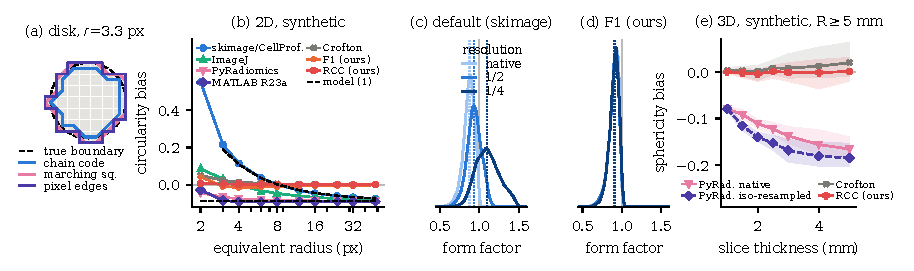
\includegraphics[width=\textwidth]{figures/fig_main.pdf}
\caption{(a) Polygons traced on a digitized disk: chain codes run inside the boundary ($\delta>0$), marching squares on it, pixel edges outside. (b) Mean circularity bias on 5{,}000 synthetic shapes vs.\ size; dashed: model, Eq.~\eqref{eq:model}. (c,d) $\ff$ of 10{,}454 BBBC038 nuclei segmented independently by Cellpose at native, $\tfrac12$ and $\tfrac14$ resolution (dotted: medians), with the default estimator (c) and F1 (d). (e) Sphericity bias of randomly rotated spheres/ellipsoids vs.\ slice thickness; bands: 10--90\% range.}
\label{fig:main}
\end{figure*}

\begin{table*}[t]
\centering\footnotesize
\caption{Real nuclei: paired shift $\Delta/\sigma$ of $\ff$ when the resolution is halved ($\tfrac12$) or quartered ($\tfrac14$), by re-digitization of the annotations (``re-dig.'') or independent Cellpose re-segmentation (``re-seg.''), and area--$\ff$ correlation $\rho_A$ at native resolution. Ideal: zero shift. OpenCV is within $0.1$ of scikit-image except at $\tfrac14$, PyRadiomics within $0.01$ of Crofton.}
\label{tab:real}
\setlength{\tabcolsep}{5pt}
\begin{tabular}{@{}l ccccc ccccc@{}}
\toprule
& \multicolumn{5}{c}{PanNuke (H\&E)} & \multicolumn{5}{c}{BBBC038 (fluorescence/brightfield)}\\
\cmidrule(lr){2-6}\cmidrule(l){7-11}
& \multicolumn{2}{c}{re-dig.} & \multicolumn{2}{c}{re-seg.} & & \multicolumn{2}{c}{re-dig.} & \multicolumn{2}{c}{re-seg.} & \\
$\ff$ from & $\tfrac12$ & $\tfrac14$ & $\tfrac12$ & $\tfrac14$ & $\rho_{A}$ & $\tfrac12$ & $\tfrac14$ & $\tfrac12$ & $\tfrac14$ & $\rho_{A}$\\
\midrule
scikit-image / CellProfiler & $+0.72$ & $+3.25$ & $+0.68$ & $+2.53$ & $-0.34$ & $+0.92$ & $+5.56$ & $+0.95$ & $+3.30$ & $-0.56$\\
ImageJ                 & $+0.34$ & $+0.96$ & $+0.31$ & $+0.96$ & $-0.21$ & $+0.41$ & $+1.31$ & $+0.48$ & $+1.68$ & $-0.41$\\
MATLAB R2023a          & $+0.06$ & $+0.27$ & $\phantom{+}0.00$ & $+0.16$ & $-0.05$ & $+0.11$ & $+0.51$ & $+0.04$ & $+0.20$ & $-0.19$\\
Crofton                & $+0.11$ & $+0.31$ & $+0.06$ & $+0.25$ & $-0.09$ & $+0.16$ & $+0.51$ & $+0.13$ & $+0.46$ & $-0.24$\\
F1 (ours, post hoc)    & $\mathbf{+0.03}$ & $\mathbf{+0.16}$ & $\mathbf{-0.03}$ & $\mathbf{+0.05}$ & $\mathbf{-0.03}$ & $\mathbf{+0.07}$ & $\mathbf{+0.35}$ & $\mathbf{-0.01}$ & $\mathbf{+0.05}$ & $\mathbf{-0.16}$\\
\bottomrule
\end{tabular}
\end{table*}

\section{Results}
\label{sec:results}
\noindent\textbf{Synthetic audit (Fig.~\ref{fig:main}b).} The chain-code tools overestimate circularity by $+0.55$ at $r=2$\,px and $+0.11$ at $r=4$\,px, cross zero near $r=8$ and underestimate it by $0.08$ at $r=48$, as Eq.~\eqref{eq:disk} predicts (dashed). ImageJ shows the same trend with a smaller range ($+0.09$ to $-0.08$). PyRadiomics and MATLAB R2023a are nearly size-independent for $r\ge3$\,px but offset by $\kappa^{-2}$ ($-0.08$ to $-0.09$); pixel edges report $0.62$ for a disk. Crofton and F1 are within $\pm0.02$ of the truth for $r\ge4$\,px.

\noindent\textbf{Resolution shifts (Fig.~\ref{fig:main}c,d; Table~\ref{tab:real}).} With the default estimator, halving the resolution shifts the mean $\ff$ by $0.7$--$0.95\sigma$ and quartering it by $2.5$--$5.6\sigma$, for re-digitized and re-segmented nuclei and both modalities; at $\tfrac14$ resolution the median BBBC038 nucleus has an impossible $\ff>1$. The default also creates an area--roundness correlation ($\rho_A=-0.34$, $-0.56$) that largely vanishes with F1 ($-0.03$, $-0.16$). Under re-segmentation, F1 reduces the shift to $|\Delta|/\sigma\le0.05$ at both resolutions, also below Crofton, whose missed short chords grow for small objects. Residual shifts under re-digitization are partly genuine, since coarse grids remove real boundary detail.

\begin{table}[t]
\centering\footnotesize
\caption{PanNuke: Cohen's $d$ of $\ff$ between nucleus types (inflammatory, connective vs.\ neoplastic; s.e.\ ${\approx}0.014$), within one magnification and when inflammatory nuclei at $20\times$ are compared with neoplastic ones at $40\times$ (``mixed''); balanced-accuracy drop of a $40\times$-trained type classifier at $10\times$ (no $\ff$: $0.008$).}
\label{tab:bio}
\setlength{\tabcolsep}{2.6pt}
\begin{tabular}{@{}lccccccc@{}}
\toprule
& \multicolumn{2}{c}{infl.--neo.} & \multicolumn{2}{c}{conn.--neo.} & mixed & drop\\
\cmidrule(lr){2-3}\cmidrule(lr){4-5}
$\ff$ from & $40\times$ & $10\times$ & $40\times$ & $10\times$ & & \\
\midrule
scikit-image / CellProfiler & $\mathbf{0.67}$ & $0.32$ & $-0.62$ & $\mathbf{+0.11}$ & $\mathbf{1.62}$ & $0.115$\\
OpenCV & $0.67$ & $0.82$ & $-0.62$ & $-0.01$ & $1.61$ & $0.106$\\
ImageJ & $0.52$ & $0.67$ & $-0.71$ & $-0.48$ & $1.05$ & $0.064$\\
PyRadiomics, Crofton & $0.40$ & $0.53$ & $-0.76$ & $-0.62$ & $0.56$ & $0.041$\\
F1 (ours) & $0.35$ & $0.39$ & $-0.79$ & $-0.41$ & $0.35$ & $0.054$\\
\bottomrule
\end{tabular}
\end{table}

\noindent\textbf{Biological contrasts (Table~\ref{tab:bio}).} Inflammatory nuclei are smaller than neoplastic ones (median radius 9.5 vs.\ 13.9\,px at $40\times$), so the default estimator inflates their apparent extra roundness from $d=0.35$--$0.40$ (size-stable estimators) to $0.67$. At $10\times$, the default reverses the sign of the connective--neoplastic contrast ($-0.62\to+0.11$). In a study that mixes scanners (inflammatory nuclei at $20\times$, neoplastic at $40\times$), the default reports $d=1.62$ instead of $0.35$ (F1), a 4.6-fold inflation. A $40\times$-trained type classifier loses $0.115$ balanced accuracy at $10\times$ with the default $\ff$ ($0.04$--$0.05$ with size-stable estimators): a biased $\ff$ turns magnification into a domain shift.

\noindent\textbf{3D (Fig.~\ref{fig:main}e).} PyRadiomics sphericity is biased by $-0.08$ at 1\,mm and $-0.17$ at 5\,mm slices; isotropic resampling before extraction, as IBSI recommends, \emph{increases} the bias to $-0.19$. The mean bias of F3 stays ${\le}0.012$ for $R\ge10$\,mm at every thickness (${\le}0.05$ at $R=5$\,mm). On the 64 lung-tumour phantoms, PyRadiomics is biased by $-0.065$ at 0.7\,mm and $-0.136$ at 5\,mm slices, F3 by $+0.005$ and $+0.042$: a 3--13$\times$ smaller error. F3's residual stems from tumour poles thinner than a slice. Re-digitizing the raw annotations instead raises the mean sphericity at 5\,mm for both estimators (PyRadiomics $0.57\to0.66$, F3 $0.63\to0.82$), because thick slices remove genuine slice-wise contour jitter.

\section{Discussion and recommendations}
\label{sec:disc}
The size dependence of the default circularity of scikit-image, CellProfiler and OpenCV is deterministic and predictable (Eq.~\eqref{eq:disk}). It distorts any comparison of objects of different pixel size. Constant-offset estimators (PyRadiomics, MATLAB R2023a, pixel edges) mislead only absolute thresholds such as ``circularity $>0.9$''. In 3D, slice thickness, a known source of radiomic variability~\cite{mali2021}, acts on IBSI sphericity through the estimator itself. We recommend: (1) Crofton perimeters for new 2D analyses; (2) F1 to repair existing CellProfiler/scikit-image tables from their Area and Perimeter columns; (3) F3 for sphericity on anisotropic volumes, on the native grid; (4) reporting object sizes in pixels. Objects below ${\sim}3$\,px radius or two slices remain unreliable for any estimator, and block-averaging images only approximates re-imaging at lower magnification. Code: \url{https://github.com/Hannibal0319/isbi2027-shape-bias}.

\section{Compliance with ethical standards}
This study uses only public, anonymized datasets; no ethical approval was required.

\section{Acknowledgments}
No funding was received; the authors have no conflicts of interest. An AI assistant (Claude, Anthropic) helped write analysis code and draft the text; all results were verified by the authors.

\bibliographystyle{IEEEbib}
\bibliography{refs}
\end{document}
